\documentclass[a4paper,12pt]{article}

\usepackage[english]{babel}
\usepackage[T1]{fontenc}
\usepackage[utf8]{inputenc}
\usepackage{amsmath}
\usepackage{amsthm}
\usepackage{graphicx}

\usepackage{geometry}
\geometry{total={210mm,297mm},
left=20mm, right=20mm,
bindingoffset=0mm,
top=20mm, bottom=20mm}

\usepackage[
  pdftitle={Homework 3},
  pdfauthor={William Jagels},
  colorlinks=true,linkcolor=blue,urlcolor=blue,citecolor=blue,bookmarks=true,
bookmarksopenlevel=2]{hyperref}

\usepackage{titlesec}
\titlelabel{\thetitle.\quad}

\def\code#1{\texttt{#1}}

\title{Homework 3}

\author{William Jagels}

\date{\today}

\begin{document}
\maketitle

\section{}
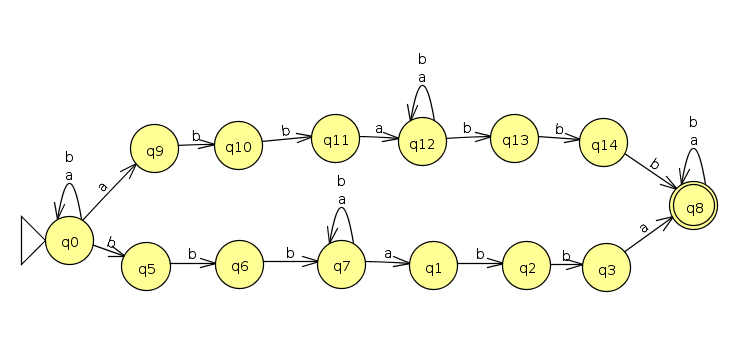
\includegraphics[width=15cm]{q1}
\section{}
\textbf{Show a language is regular if and only if there is an all-NFA that recognizes it.}
Assume that:
1. A language is regular if and only if a DFA recognizes it;
2. A language is regular if and only if an NFA recognizes it.

Any DFA is equivalent to an all-NFA since DFAs only have one state they can be in anyways.
An all-NFA can also be converted into a DFA using the same methodology as with an NFA.
Therefore, by the transitive property, a language is regular if and only if there is an all-NFA that recognizes it.
\section{}
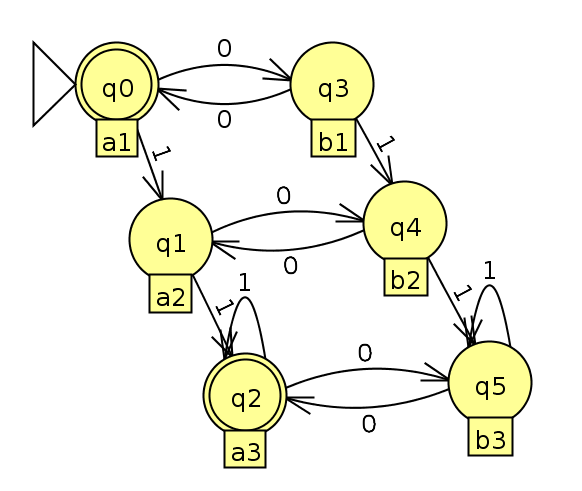
\includegraphics[width=15cm]{q3}
\section{}
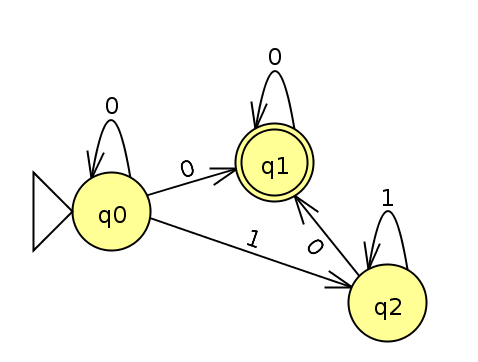
\includegraphics[width=15cm]{q4}
\section{}
\textbf{When we showed that the class of regular languages is closed under complementation, we took
a DFA and swapped the accept and non-accept states. Does the same construction work for an
NFA? If it does, prove it. If it doesn't, give a counter example.}

This doesn't work.
See counter-example.
The first NFA accepts all strings over $0,1$ ending in $00$.
Flipping the states results in an NFA that accepts all strings over $0,1$

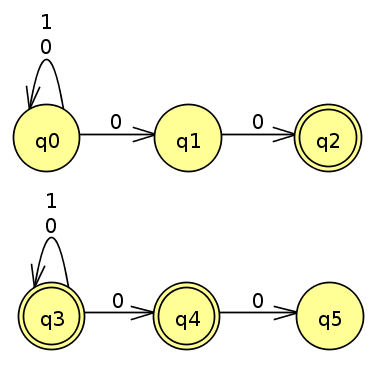
\includegraphics[width=5cm]{q5}
\section{}
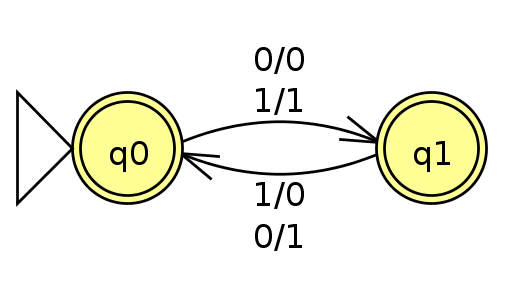
\includegraphics[width=15cm]{q6}
\section{}
\textbf{For languages A, B, and C, define the extended perfect shuffle of A, B, and C as the
language} $\{ w | w = a_1 b_1 c_1 \ldots a_n b_n c_n,$ with $a_1 \ldots a_n$ in $A, b_1 \ldots b_n$ in $B,$ and $c_1 \ldots c_n$ in $C \}$.
\textbf{Show that the class of regular languages is closed under the extended perfect shuffle.
The extended perfect shuffle is a minor modification of the perfect shuffle defined in “Introduction to the Theory of Computation”, Michael Sipser.}

To show this, we need construct an NFA that will recognize the perfect shuffle of three languages.
We can do this by constructing three NFAs that recognize languages A, B, and C.
Then, to recognize all of the languages, we can add $\epsilon$-transitions between each of the NFAs to the others.

\section{}
\textbf{For languages A and B, let the shuffle of A and B be the language}
\{$w| w = a_1 b_1 \cdots a_k b_k,$ where $a_1 \cdots a_k \in A$ and $b_1 \cdots b_k \in B,$ each $a_i , b_i \in \Sigma^* $\}.
\textbf{Show that the class of regular languages is closed under shuffle.}

To show this, we need construct an NFA that will recognize the shuffle of two languages.
We can do this by constructing three NFAs that recognize languages A and B.
Then, to recognize all of the languages, we can add $\epsilon$-transitions between each of the NFAs to the others.


\section{}
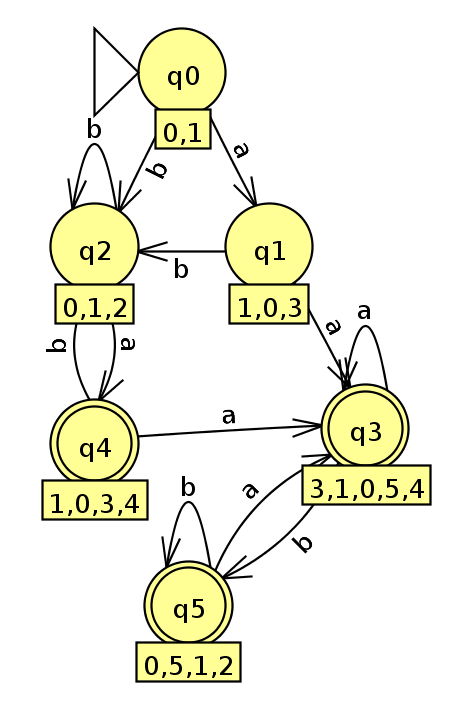
\includegraphics[width=10cm]{q9}
\section{}
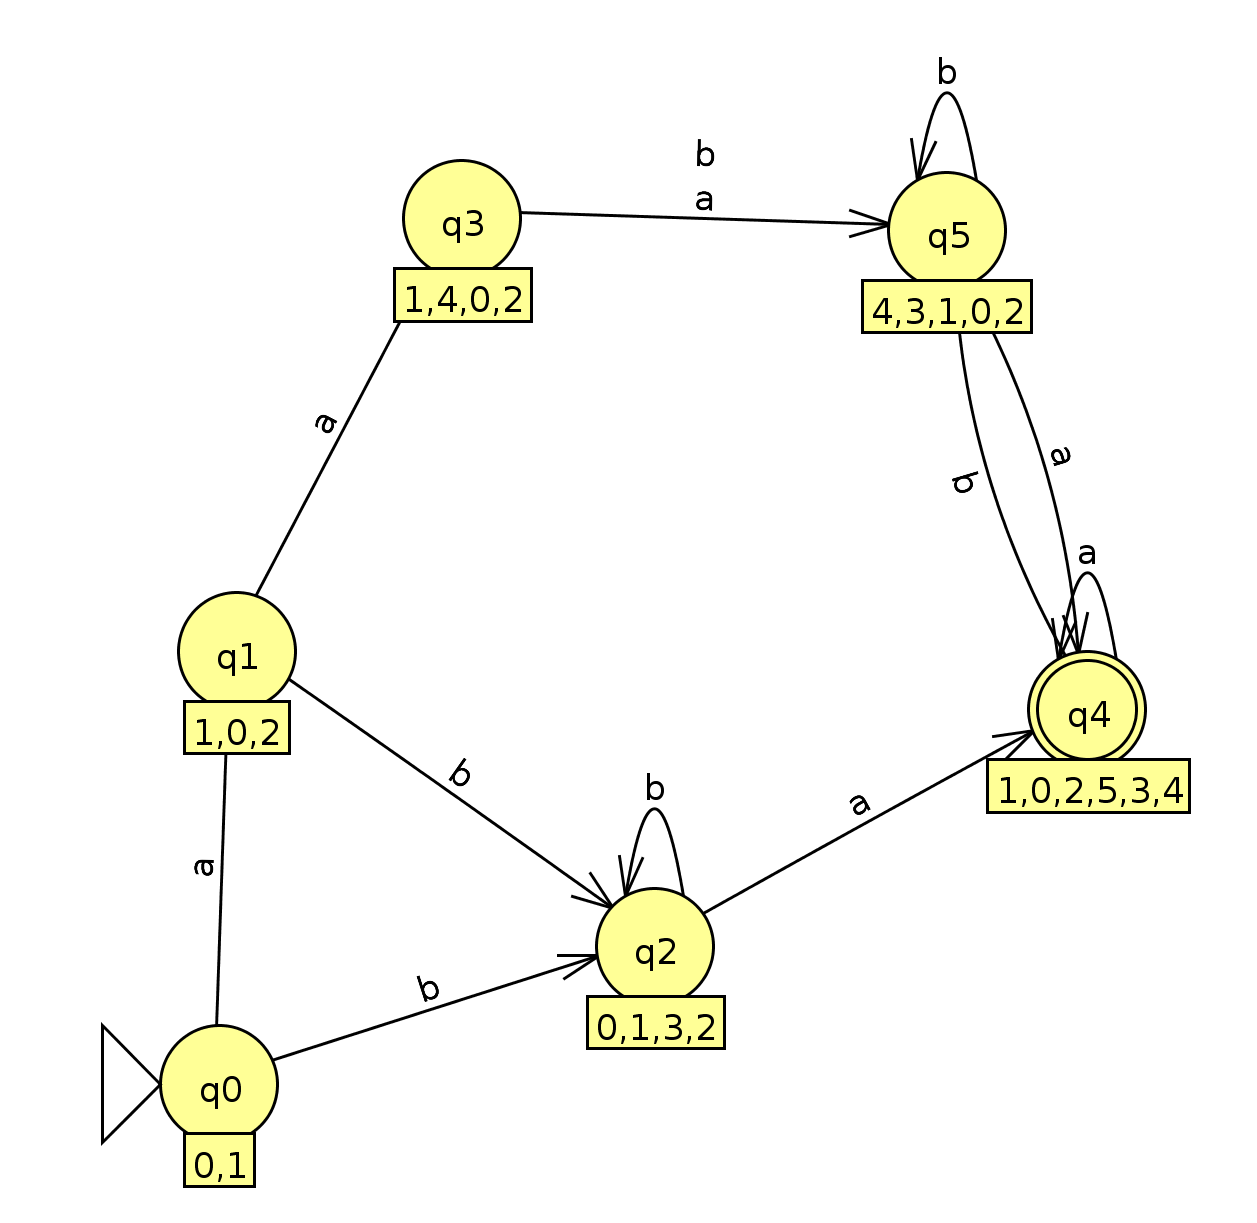
\includegraphics[width=15cm]{q10}

\end{document}
